\chapter{STP Tree Generator}
\label{stp_gen}
We split the application in three parts:
\begin{itemize}
    \item \textbf{Client}: collects STP information and sends it to the server.
        The client also handles piecing together the packets into paths.
    \item \textbf{Server}: saves the data from the clients and combines them into one tree.
    \item \textbf{Parser}: contacts the server to receive the tree and converts it into output format.
\end{itemize}
The intended form of usage is to have multiple clients in the network connecting to one server.
We combine information received from multiple clients to reach a better understanding of the network.

STP uses only local data, which means that bridges have no knowledge of the network, except for their own port states.
Unfortunately for us, this means that it is hard to find connections between bridges.
The only way to obtain this information is to capture packets during the tree build up.

When the client witnesses the message age increasing by one, it assumes that the new root should be prepended to the previous one.
This assumption is unsafe, as this connection cannot be guaranteed, but the risk of making mistakes can be reduced.
Details on this are discussed in the section on unsafe assumptions (Section~\ref{unsafe_assumptions})
Figure~\ref{fig:build_up} shows a rudimentary example of information gained during tree build up.
%TODO: check that the figures don't break any listings
\begin{figure}[p]
    \begin{centering}
        \begin{subfigure}[b]{0.4\textwidth}
            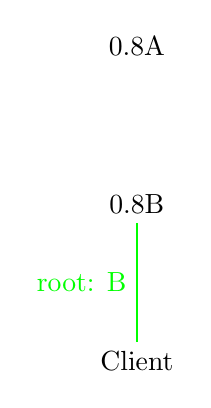
\begin{tikzpicture}
                \node (a) at (4,4) {\switch{0.8}{A}};
                \node (b) at (4,2) {\switch{0.8}{B}};
                \node (client) at (4,0) {Client};

                \draw[green, thick]
                (b) -- node [left] {root: B} ++ (client);

            \end{tikzpicture}
            \caption{B thinks it is root}
        \end{subfigure}
        \hspace{1cm}
        \begin{subfigure}[b]{0.4\textwidth}
            \centering
            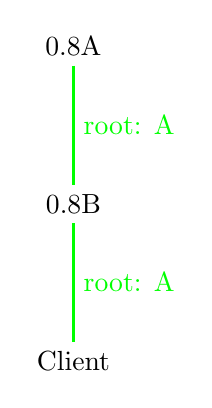
\begin{tikzpicture}
                \node (a) at (4,4) {\switch{0.8}{A}};
                \node (b) at (4,2) {\switch{0.8}{B}};
                \node (client) at (4,0) {Client};

                \draw[green, thick]
                (a) -- node [right] {root: A} ++ (b);
                \draw[green, thick] 
                (b) -- node [right] {root: A} ++ (client);
            \end{tikzpicture}
            \caption{Root information updated}
        \end{subfigure}
    \end{centering}
    \caption{Information gained on STP build up}
    \label{fig:build_up}
\end{figure}

Unfortunately, this works only if the message age increases by one at the same time that the root changes.
For other cases there are simply too many cases to assume a certain change with a reasonable safety.%TODO: source?
Figure \ref{fig:information_lost} shows an example case where the client has to reset its data.
A detailed explanation of how this tool handles incoming STP packets can be found in the section on packet handling (Section~\ref{packet_handling}).

\begin{figure}[p]
    \begin{centering}
        \begin{subfigure}[b]{0.4\textwidth}
            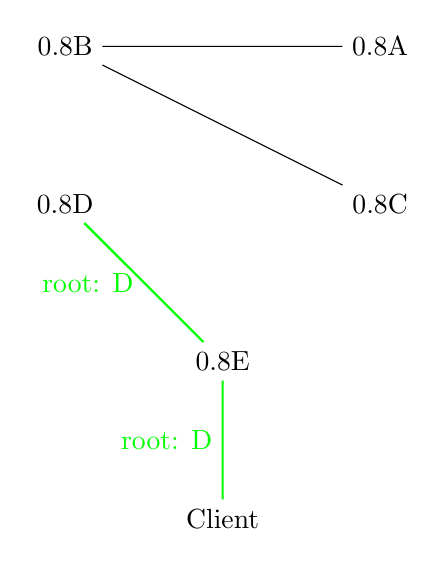
\begin{tikzpicture}
                \node (a) at (6,6) {\switch{0.8}{A}};
                \node (b) at (2,6) {\switch{0.8}{B}};
                \node (c) at (6,4) {\switch{0.8}{C}};
                \node (d) at (2,4) {\switch{0.8}{D}};
                \node (e) at (4,2) {\switch{0.8}{E}};
                \node (client) at (4,0) {Client};
                \draw
                (a) -- (b)
                (b) -- (c);
                \draw[green, thick]
                (d) -- node [left] {root: D} ++ (e)
                (e) -- node [left] {root: D} ++ (client);
            \end{tikzpicture}
            \caption{Some information known}
        \end{subfigure}
        \hspace{1cm}
        \begin{subfigure}[b]{0.4\textwidth}
            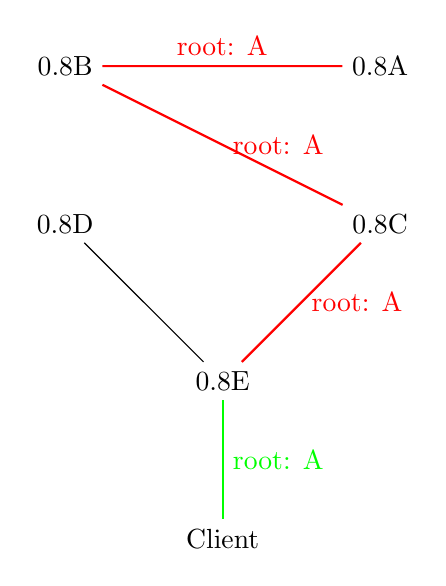
\begin{tikzpicture}
                \node (a) at (6,6) {\switch{0.8}{A}};
                \node (b) at (2,6) {\switch{0.8}{B}};
                \node (c) at (6,4) {\switch{0.8}{C}};
                \node (d) at (2,4) {\switch{0.8}{D}};
                \node (e) at (4,2) {\switch{0.8}{E}};
                \node (client) at (4,0) {Client};
                \draw
                (d) -- (e);
                \draw[green, thick]
                (e) -- node [right] {root: A} ++ (client);
                \draw[red, thick]
                (a) -- node [above] {root: A} ++ (b)
                (b) -- node [right] {root: A} ++ (c)
                (c) -- node [right] {root: A} ++ (e);
            \end{tikzpicture}
            \caption{Previous information lost}
        \end{subfigure}
        \caption{Information lost during tree build up}
        \label{fig:information_lost}
    \end{centering}
\end{figure}

\section{Details}
\subsection{Class Structure}
\label{data}
We created multiple classes to make saving the STP data easier, as well as reduce the effort needed to generate \textit{JSON} and \textit{TikZ} output.
There are classes to represent MAC addresses, bridges, and complete spanning trees.
All these classes have conversion functions from and to \textit{JSON} format, as well as a function to generate \textit{TikZ} output.
Altogether the following classes were created:
\begin{itemize}
    \item \textbf{Mac}: A container class for MAC addresses.
        It is used to store the address in nicer format.
    \item \textbf{Bridge}: Stores a \textbf{MAC} object in conjunction with the priority and message age.
    \item \textbf{SpanningTree}: This class represents an entire tree.
        It has functions for creating the \textit{TikZ} export as well as combining and manipulating subtrees.
    \item \textbf{Sniffer}: Does the actual packet sniffing.
    \item \textbf{Client}: Handle the client side communication.
    \item \textbf{Server}: Handles the server side communication, as well as combining the trees and removing incorrect information.
\end{itemize}
The STP data is saved in the \textbf{Sniffer} as a vector.
This is easier than storing them in a fixed size array, and already combining them into a \textbf{SpanningTree} object would keep the server from performing the steps described in Section~\ref{unsafe_assumptions}

\subsection{Packet Handling}
\label{packet_handling}
Packets are handled by the sniffer class.
While the function mostly skips unused fields in the STP packet, here we will take a close look at the more important parts.
In order to check if the packet is actually an STP packet, we use the Ethernet destination address.
Listing~\ref{lst:filter} shows how that is done.
The \textit{bytes} variable is provided by the required \textit{pcap} callback prototype (see Section~\ref{pcap}: PCAP).
This way is computationally more expensive than saving the destination in binary format and comparing memory.
It is however also more readable and a lot easier to change should the need arise.
%TODO: check capitalization in captions
\lstinputlisting[caption=Filtering for STP packets, label=lst:filter]{../listings/stp/stpFilter.c}

\textit{Pcap} provides us with a pointer to the binary packet data.
We can go through the packet by incrementing this pointer by set amounts (after skipping to the STP data).
This repeats for the bridge identifier, as well as other fields.
Listing~\ref{lst:payload} shows the beginning of the payload handling.
\lstinputlisting[caption=Going Through the Payload, label=lst:payload]{../listings/stp/payload.c}

After the data is extracted from the packet, it is constructed into our custom classes.
We then check if the two bridges (root and first hop) were previously known, as seen in Listing~\ref{lst:contained}.
Concerning the root, knowing whether or not it was previously known is enough.
For the first hop, we also require knowledge about the old message age.
\lstinputlisting[caption=Checking for previously known information, label= lst:contained]{../listings/stp/contained.c}

Listing~\ref{lst:update} shows how we update the bridge information in the sniffer.
The \textit{clearAndAdd} function is just a shorthand to clear the bridge vector before adding the two bridges to it.
\lstinputlisting[caption=Bridge data update, label=lst:update]{../listings/stp/update.c}
\subsection{Communication}
\label{communication}
As discussed in the background section (Section~\ref{json}) wer are using JSON for the client server communication.
To inform all involved components about the purpose of a JSON message, we use a \textit{messagetype} field.
The possibilities for \textit{messagetypes} are as follows:
\begin{itemize}
    \item \textbf{Register}: before they can send data to the server, the clients need to register to receive an identifier.
        These unique identifiers are used to keep the data from different clients separated.
    \item \textbf{Push}: clients send \textit{push} messages when they transmit their data to the server.
        These messages contain lists of bridges.
        They are transmitted the same way that they are stored in the sniffer, without modifications.
    \item \textbf{Report}: the parser sends a message to the server containing this \textit{messagetype} and nothing else.
        The server then combines the client data and transmits it to the parser.
\end{itemize}
Bridge data is transmitted from the client to the server in standard JSON array notation.
When the data is transmitted from the server to the parser, it is transmitted as a full tree.
We added conversion functions to and from JSON to all our custom data classes, to keep this transmission simple.
Listing~\ref{lst:arrayJson} shows an example transmission from client to server, and Listing~\ref{lst:treeJson} shows a transmission from server to parser.
The JSON tree shown in Listing~\ref{lst:treeJson} the tree resulting from our test runs.
It shows how the tool can use changing packets to gather information about bridge connections.
\lstinputlisting[caption=Client-Server Transmission, label=lst:arrayJson]{../listings/json/clientServer.json}
%TODO: check positioning of listings on pages (especially large json)
\lstinputlisting[caption=Server-Parser Transmission, label=lst:treeJson]{../listings/json/serverParser.json}

\subsection{Unsafe Assumptions}
\label{unsafe_assumptions}
As previously said, the assumptions we make about bridge connections are not necessarily true.
They can be wrong, for certain cases, one of which is shown in Figure~\ref{fig:false_example}.
\begin{figure}[h]
    \begin{subfigure}[b]{0.4\textwidth}
        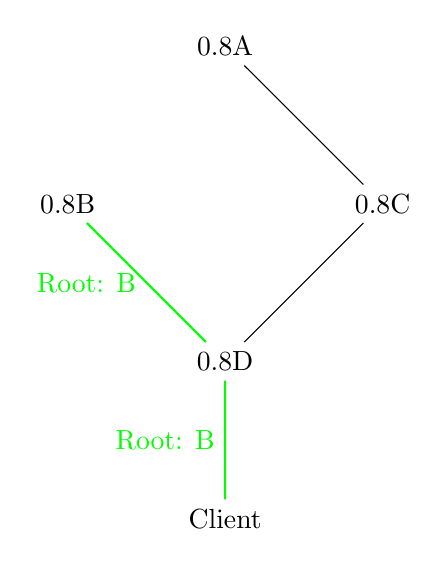
\begin{tikzpicture}
            \node (A) at (4,8) {\switch{0.8}{A}};
            \node (B) at (2,6) {\switch{0.8}{B}};
            \node (C) at (6,6) {\switch{0.8}{C}};
            \node (D) at (4,4) {\switch{0.8}{D}};
            \node (client) at (4,2) {Client};

            \draw
            (A) -- (C)
            (C) -- (D);

            \draw[green, thick]
            (B) -- node [left] {Root: B} ++ (D)
            (D) -- node [left] {Root: B} ++ (client);
        \end{tikzpicture}
        \caption{Correct information}
    \end{subfigure}
    \hspace{1cm}
    \begin{subfigure}[b]{0.4\textwidth}
        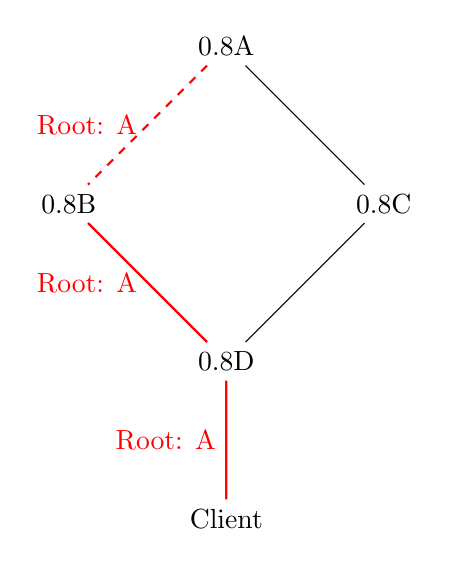
\begin{tikzpicture}
            \node (A) at (4,8) {\switch{0.8}{A}};
            \node (B) at (2,6) {\switch{0.8}{B}};
            \node (C) at (6,6) {\switch{0.8}{C}};
            \node (D) at (4,4) {\switch{0.8}{D}};
            \node (client) at (4,2) {Client};

            \draw
            (A) -- (C)
            (C) -- (D);

            \draw[red, thick]
            (B) -- node [left] {Root: A} ++ (D)
            (D) -- node [left] {Root: A} ++ (client);

            \draw[red, thick, dashed]
            (A) -- node [left] {Root: A} ++ (B);
        \end{tikzpicture}
        \caption{False assumption}
    \end{subfigure}

    \caption{An example case of false assumptions about network structure}
    \label{fig:false_example}
\end{figure}
We did not find an alternate way to gather information about connections in the network, so we tried to reduce errors created by our method.
To this end we combine information gathered by multiple clients to identify and remove false information.
If a client makes a false assumption about a bridge, the message age for that bridge will be lower than its actual messge age.
An example can be seen in Figure~\ref{fig:message_ages}.
\begin{figure}[h]
    \begin{subfigure}[b]{0.4\textwidth}
        \begin{tikzpicture}
            \node (A) at (4,8) {\switch{0.8}{A:0}};
            \node (B) at (2,6) {\switch{0.8}{B:1}};
            \node (C) at (6,6) {\switch{0.8}{C:1}};
            \node (D) at (4,4) {\switch{0.8}{D:2}};
            \node (client) at (4,2) {Client};

            \draw
            (A) -- (C)
            (C) -- (D)
            (B) -- (D)
            (D) -- (client);

            \draw [red, thick, dashed]
            (A) -- (B);

        \end{tikzpicture}
        \caption{Assumed message ages}
    \end{subfigure}
    \hspace{1cm}
    \begin{subfigure}[b]{0.4\textwidth}
        \begin{tikzpicture}
            \node (A) at (4,8) {\switch{0.8}{A: 0}};
            \node (B) at (2,6) {\switch{0.8}{B: 3}};
            \node (C) at (6,6) {\switch{0.8}{C: 1}};
            \node (D) at (4,4) {\switch{0.8}{D: 2}};
            \node (client) at (4,2) {Client};

            \draw
            (A) -- (C)
            (C) -- (D)
            (B) -- (D)
            (D) -- (client);

        \end{tikzpicture}
        \caption{Actual message ages}
    \end{subfigure}

    \caption{Assumed and actual message ages}
    \label{fig:message_ages}
\end{figure}
By comparing bridge data from multiple clients we can find and remove bridges whose message age is lower than it should be.
The code for doing this is shown in Listing~\ref{lst:remove}.
\lstinputlisting[caption=Removing false bridge data, label=lst:remove]{../listings/stp/remove.c} %TODO: maybe do better formatting
The bridges are removed from the vector they each are in.
This way any connection information that is not proven wrong is retained.
\subsection{Combining the data}
\label{combining_data}
After false information is removed, the bridge data is combined into one SpanningTree object.
Creating large SpanningTree objects is done in multiple steps.
First, we combine the bridge vectors to individual trees.
These trees each represent a path from a client to the root.
After the individual trees are obtained, we combine the ones with the same root.
The code for this can be seen in Listing~\ref{lst:combine}.
\lstinputlisting[caption=Combining the bridge data, label=lst:combine]{../listings/stp/combination.c}

\section{Installation \& Usage}
%TODO: extend this section?
%TODO: talk about the fact that it is C++
The tool requires \textit{pcap} and \textit{jsoncpp} at build time.
We packaged the version of \textit{jsoncpp} we use, so to build the tool only \textit{pcap} needs to be installed.
The library can be found in the repository for most package managers, as well as on GitHub\cite{tcpdump_git}.

For a manual on configuration files and launch parameters please consult the README file found in our git\cite{stp_git}.
